\documentclass[11pt,a4paper]{article}
\usepackage{amsmath}
\usepackage{amsfonts}
\usepackage{amssymb}
\usepackage{makeidx}
\usepackage{graphicx}
\usepackage{wrapfig}
\usepackage{enumerate}
\usepackage{pdfpages}
\usepackage{tocloft}
\usepackage{setspace}
\usepackage{mathtools}
\usepackage{hyperref}
\definecolor{linkcolour}{rgb}{0,0.2,0.6} % Link color
\hypersetup{colorlinks,breaklinks,urlcolor=linkcolour,linkcolor=linkcolour}

\usepackage[left=2cm,right=2cm,top=2cm,bottom=2cm]{geometry}

\usepackage{xcolor}

\usepackage{fontspec}
\setmainfont{Cambria}

\usepackage{caption}
\captionsetup[figure]{font=small, labelfont={bf}}
\captionsetup[table]{font=small, labelfont={bf}}

\usepackage{float}
\usepackage{multirow}
\usepackage{longtable}

\usepackage[nottoc]{tocbibind}

\newcommand{\spa}{\vspace{1.25em}}
\newcommand{\noi}{\noindent}
\def\dul#1{\underline{\underline{#1}}}
\def\cpt#1#2{{\begin{center}\small\textbf{\textcolor{blue}{Figure #1:}} #2\end{center}}}
\def\tt#1{\texttt{#1}}

% for dots in the content
\usepackage{tocloft}
\renewcommand{\cftsecleader}{\cftdotfill{\cftdotsep}}

\begin{document}
	\begin{titlepage} 
		\begin{center}
		\large{ASSIGNMENT 2}\\
		\vspace{2em}
		\large {CS5691 Pattern Recognition and Machine Learning}
		\vspace{3em}
		
		\rule{0.9\linewidth}{0.5mm} \\[0.4cm]
	    {\Large{\bfseries{CS5691 Assignment 2}}} \\
	    \rule{0.9\linewidth}{0.5mm} \\[3 em]	
	    
	    Team Members: \\
	    \vspace{0.5em}
	   	\def\arraystretch{1.25}
\begin{tabular}{c l}
	\hline
	BE17B007 & N Sowmya Manojna \\
	PH17B010 & Thakkar Riya Anandbhai \\
	PH17B011 & Chaithanya Krishna Moorthy \\
	\hline
\end{tabular}

		\vspace{1em}

		Indian Institute of Technology, Madras\\    
		
		\vspace{5em}    
	    
	    	
\includegraphics[scale = 0.09]{images/iitmlogo.png}
		\end{center}
	\end{titlepage}

{\hypersetup{linkcolor=black}
 \tableofcontents}
\break


\section{Dataset 1A}
\subsection{K-nearest Neighbors Classifier}
\subsection{Naive-Bayes classifier}
\subsubsection{Same Covariance Matrix ($\sigma^2I$)}
\subsubsection{Same Covariance Matrix ($C$)}
\subsubsection{Different Covariance Matrix}

\break
\section{Dataset 1B}
\subsection{K-nearest Neighbors Classifier}
\subsection{Bayes Classifier, GMM, full covariance}
Based on the accuracies obtained on the training, validation and test dataset, the best $q_i$ for the three classes has been chosen as $5$.
\subsubsection{Training and Validation Accuracy}
The training and validation accuracies obtained for varying $q_i$ for each class is as follows:
\begin{figure}[H]
    \hspace{-2em}
    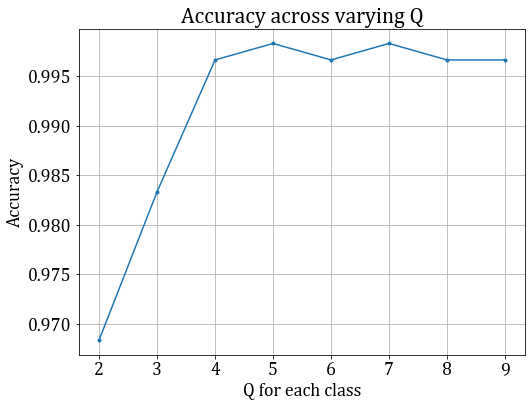
\includegraphics[scale=0.5]{images/1b_full_train.png}
    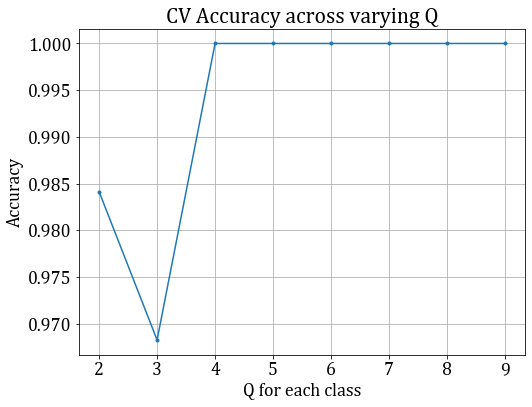
\includegraphics[scale=0.5]{images/1b_full_val.png}
    \caption{Training and Validation accuracy across $q_i$, on the left and right respectively}
\end{figure}

\subsubsection{Testing Accuracy}
The testing accuracy obtained for varying $q_i$ for each class is as follows:
\begin{figure}[H]
    \centering
    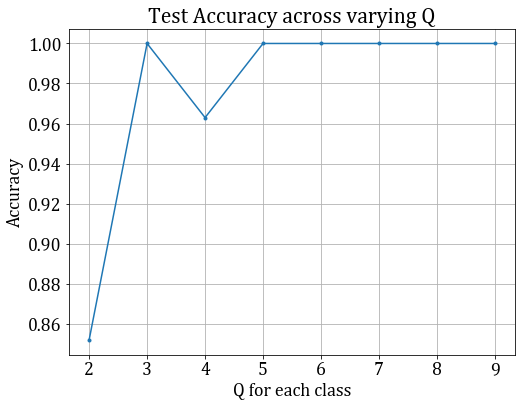
\includegraphics[scale=0.5]{images/1b_full_test.png}
    \caption{Testing accuracy across $q_i$}
\end{figure}

\subsubsection{Contour Maps and Decision Surfaces}
The contour maps and decision surfaces obtained, with $q_i=5$ are as follows:
\begin{figure}[H]
    \hspace{-1em}
    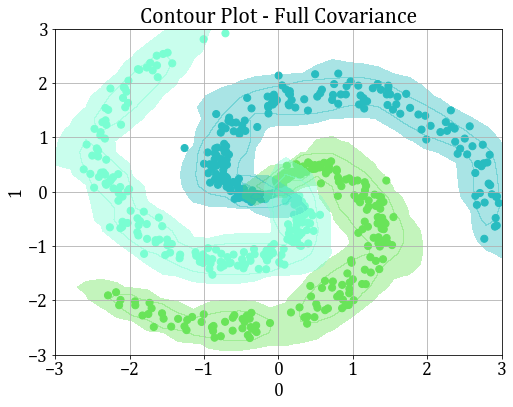
\includegraphics[scale=0.5]{images/1b_full_contours.png}
    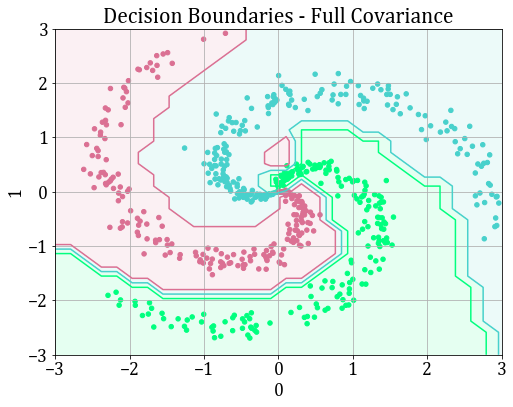
\includegraphics[scale=0.5]{images/1b_full_decision_surfaces.png}
    \caption{Contour Maps and Decision Surfaces obtained for $q_i=5$, on the left and right respectively}
\end{figure}


\subsection{Bayes Classifier, GMM, diagonal covariance}
\subsection{Bayes Classifier, KNN}

\break
\section{Dataset 2A}
\subsection{Bayes Classifier, GMM, full covariance}
\subsection{Bayes Classifier, GMM, diagonal covariance}

\break
\section{Dataset 2B}
\subsection{Bayes Classifier, GMM, full covariance}
\subsection{Bayes Classifier, GMM, diagonal covariance}

\end{document}